\documentclass[14pt]{extbook}
\usepackage{multicol, enumerate, enumitem, hyperref, color, soul, setspace, parskip, fancyhdr} %General Packages
\usepackage{amssymb, amsthm, amsmath, bbm, latexsym, units, mathtools} %Math Packages
\everymath{\displaystyle} %All math in Display Style
% Packages with additional options
\usepackage[headsep=0.5cm,headheight=12pt, left=1 in,right= 1 in,top= 1 in,bottom= 1 in]{geometry}
\usepackage[usenames,dvipsnames]{xcolor}
\usepackage{dashrule}  % Package to use the command below to create lines between items
\newcommand{\litem}[1]{\item#1\hspace*{-1cm}\rule{\textwidth}{0.4pt}}
\pagestyle{fancy}
\lhead{Progress Quiz 4}
\chead{}
\rhead{Version C}
\lfoot{8448-1521}
\cfoot{}
\rfoot{Fall 2020}
\begin{document}

\begin{enumerate}
\litem{
Solve the linear equation below. Then, choose the interval that contains the solution.\[ \frac{8x -9}{8} - \frac{-3x + 9}{2} = \frac{-7x -3}{7} \]\begin{enumerate}[label=\Alph*.]
\item \( x \in [-1.5, -0.3] \)
\item \( x \in [-0.4, 0.6] \)
\item \( x \in [1.3, 1.7] \)
\item \( x \in [2.5, 4.4] \)
\item \( \text{There are no real solutions.} \)

\end{enumerate} }
\litem{
First, find the equation of the line containing the two points below. Then, write the equation as $ y=mx+b $ and choose the intervals that contain $m$ and $b$.\[ (11, 3) \text{ and } (3, -6) \]\begin{enumerate}[label=\Alph*.]
\item \( m \in [-0.5, 6.1] \hspace*{3mm} b \in [-9.71, -9.24] \)
\item \( m \in [-0.5, 6.1] \hspace*{3mm} b \in [-8.01, -7.97] \)
\item \( m \in [-0.5, 6.1] \hspace*{3mm} b \in [-9.36, -8.5] \)
\item \( m \in [-0.5, 6.1] \hspace*{3mm} b \in [9.18, 9.42] \)
\item \( m \in [-6.1, -0.2] \hspace*{3mm} b \in [-2.99, -2.62] \)

\end{enumerate} }
\litem{
First, find the equation of the line containing the two points below. Then, write the equation as $ y=mx+b $ and choose the intervals that contain $m$ and $b$.\[ (-3, 11) \text{ and } (10, -7) \]\begin{enumerate}[label=\Alph*.]
\item \( m \in [-3.4, 0.5] \hspace*{3mm} b \in [-17.2, -15.7] \)
\item \( m \in [-3.4, 0.5] \hspace*{3mm} b \in [11.8, 15.4] \)
\item \( m \in [-3.4, 0.5] \hspace*{3mm} b \in [-7.5, -5.1] \)
\item \( m \in [-3.4, 0.5] \hspace*{3mm} b \in [2.9, 7.9] \)
\item \( m \in [-0.3, 3.4] \hspace*{3mm} b \in [-21.5, -19.3] \)

\end{enumerate} }
\litem{
Solve the equation below. Then, choose the interval that contains the solution.\[ -7(8x + 11) = -13(10x -5) \]\begin{enumerate}[label=\Alph*.]
\item \( x \in [-0.14, 0.01] \)
\item \( x \in [1.72, 2.08] \)
\item \( x \in [-0.26, -0.13] \)
\item \( x \in [0.09, 0.49] \)
\item \( \text{There are no real solutions.} \)

\end{enumerate} }
\litem{
Write the equation of the line in the graph below in Standard form $Ax+By=C$. Then, choose the intervals that contain $A, B, \text{ and } C$.
\begin{center}
    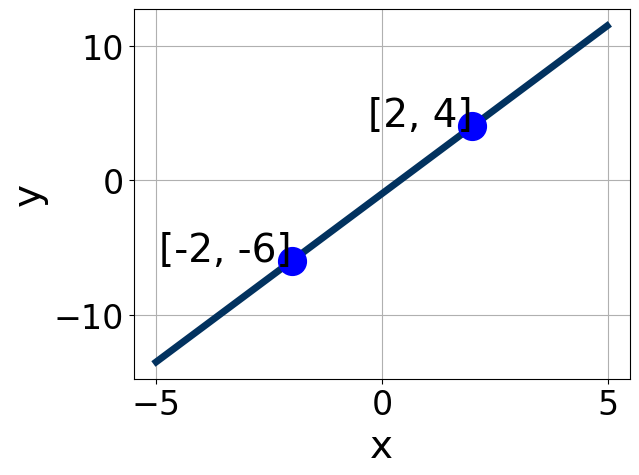
\includegraphics[width=0.5\textwidth]{../Figures/linearGraphToStandardCopyC.png}
\end{center}
\begin{enumerate}[label=\Alph*.]
\item \( A \in [-5, -4], \hspace{3mm} B \in [3.8, 6.8], \text{ and } \hspace{3mm} C \in [14, 23] \)
\item \( A \in [-1.25, 0.75], \hspace{3mm} B \in [-2, -0.1], \text{ and } \hspace{3mm} C \in [-8, -2] \)
\item \( A \in [-1, 7], \hspace{3mm} B \in [3.8, 6.8], \text{ and } \hspace{3mm} C \in [14, 23] \)
\item \( A \in [-1.25, 0.75], \hspace{3mm} B \in [-0.3, 3.4], \text{ and } \hspace{3mm} C \in [0, 6] \)
\item \( A \in [-1, 7], \hspace{3mm} B \in [-4.4, -3.1], \text{ and } \hspace{3mm} C \in [-21, -15] \)

\end{enumerate} }
\litem{
Solve the linear equation below. Then, choose the interval that contains the solution.\[ \frac{7x + 8}{5} - \frac{-7x -3}{4} = \frac{8x + 9}{3} \]\begin{enumerate}[label=\Alph*.]
\item \( x \in [-5.41, -3.61] \)
\item \( x \in [-0.01, 0.42] \)
\item \( x \in [0.63, 1.89] \)
\item \( x \in [3.37, 4.72] \)
\item \( \text{There are no real solutions.} \)

\end{enumerate} }
\litem{
Write the equation of the line in the graph below in Standard form $Ax+By=C$. Then, choose the intervals that contain $A, B, \text{ and } C$.
\begin{center}
    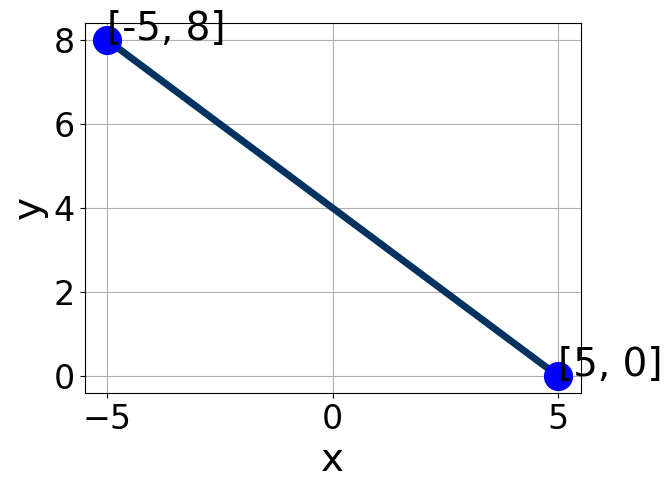
\includegraphics[width=0.5\textwidth]{../Figures/linearGraphToStandardC.png}
\end{center}
\begin{enumerate}[label=\Alph*.]
\item \( A \in [-1.5, 1.2], \hspace{3mm} B \in [0.3, 3.6], \text{ and } \hspace{3mm} C \in [4, 6] \)
\item \( A \in [2.6, 5.1], \hspace{3mm} B \in [4.4, 5.3], \text{ and } \hspace{3mm} C \in [19, 26] \)
\item \( A \in [2.6, 5.1], \hspace{3mm} B \in [-5.2, -3.9], \text{ and } \hspace{3mm} C \in [-20, -12] \)
\item \( A \in [-1.5, 1.2], \hspace{3mm} B \in [-3, -0.2], \text{ and } \hspace{3mm} C \in [-5, 2] \)
\item \( A \in [-7.2, -1.1], \hspace{3mm} B \in [-5.2, -3.9], \text{ and } \hspace{3mm} C \in [-20, -12] \)

\end{enumerate} }
\litem{
Find the equation of the line described below. Write the linear equation as $ y=mx+b $ and choose the intervals that contain $m$ and $b$.\[ \text{Parallel to } 5 x + 8 y = 7 \text{ and passing through the point } (6, 8). \]\begin{enumerate}[label=\Alph*.]
\item \( m \in [-0.75, -0.53] \hspace*{3mm} b \in [-17.75, -5.75] \)
\item \( m \in [0.16, 1.85] \hspace*{3mm} b \in [4.25, 6.25] \)
\item \( m \in [-1.96, -1.14] \hspace*{3mm} b \in [10.75, 12.75] \)
\item \( m \in [-0.75, -0.53] \hspace*{3mm} b \in [10.75, 12.75] \)
\item \( m \in [-0.75, -0.53] \hspace*{3mm} b \in [-2, 4] \)

\end{enumerate} }
\litem{
Find the equation of the line described below. Write the linear equation as $ y=mx+b $ and choose the intervals that contain $m$ and $b$.\[ \text{Perpendicular to } 9 x - 7 y = 12 \text{ and passing through the point } (-5, 3). \]\begin{enumerate}[label=\Alph*.]
\item \( m \in [-1.2, 0.3] \hspace*{3mm} b \in [7.43, 8.13] \)
\item \( m \in [-0.7, 2.2] \hspace*{3mm} b \in [6.27, 6.95] \)
\item \( m \in [-1.2, 0.3] \hspace*{3mm} b \in [0.42, 1.3] \)
\item \( m \in [-1.7, -0.9] \hspace*{3mm} b \in [-1.38, -0.12] \)
\item \( m \in [-1.2, 0.3] \hspace*{3mm} b \in [-1.38, -0.12] \)

\end{enumerate} }
\litem{
Solve the equation below. Then, choose the interval that contains the solution.\[ -7(19x + 17) = -15(-18x + 9) \]\begin{enumerate}[label=\Alph*.]
\item \( x \in [-0.76, -0.25] \)
\item \( x \in [-0.27, 0.14] \)
\item \( x \in [0.61, 0.67] \)
\item \( x \in [1.26, 1.92] \)
\item \( \text{There are no real solutions.} \)

\end{enumerate} }
\end{enumerate}

\end{document}